\documentclass[fleqn,10pt]{wlscirep}
\usepackage[utf8]{inputenc}
\usepackage[T1]{fontenc}
\usepackage[section]{placeins}
\usepackage{amsmath}
\usepackage{lineno}
\usepackage{float}
\usepackage{booktabs}
\usepackage{longtable}
\usepackage{array}
\usepackage{multirow}
\usepackage{wrapfig}
\usepackage{colortbl}
\usepackage{pdflscape}
\usepackage{tabu}
\usepackage{threeparttable}
\usepackage{threeparttablex}
\usepackage[normalem]{ulem}
\usepackage{makecell}
\usepackage{xcolor}
\usepackage{hyperref}
\usepackage{bookmark}
\linenumbers

\urlstyle{same}

\providecommand{\tightlist}{%
  \setlength{\itemsep}{0pt}\setlength{\parskip}{0pt}}

\usepackage{color}
\usepackage{fancyvrb}
\newcommand{\VerbBar}{|}
\newcommand{\VERB}{\Verb[commandchars=\\\{\}]}
\DefineVerbatimEnvironment{Highlighting}{Verbatim}{commandchars=\\\{\}}
% Add ',fontsize=\small' for more characters per line
\usepackage{framed}
\definecolor{shadecolor}{RGB}{248,248,248}
\newenvironment{Shaded}{\begin{snugshade}}{\end{snugshade}}
\newcommand{\AlertTok}[1]{\textcolor[rgb]{0.94,0.16,0.16}{#1}}
\newcommand{\AnnotationTok}[1]{\textcolor[rgb]{0.56,0.35,0.01}{\textbf{\textit{#1}}}}
\newcommand{\AttributeTok}[1]{\textcolor[rgb]{0.77,0.63,0.00}{#1}}
\newcommand{\BaseNTok}[1]{\textcolor[rgb]{0.00,0.00,0.81}{#1}}
\newcommand{\BuiltInTok}[1]{#1}
\newcommand{\CharTok}[1]{\textcolor[rgb]{0.31,0.60,0.02}{#1}}
\newcommand{\CommentTok}[1]{\textcolor[rgb]{0.56,0.35,0.01}{\textit{#1}}}
\newcommand{\CommentVarTok}[1]{\textcolor[rgb]{0.56,0.35,0.01}{\textbf{\textit{#1}}}}
\newcommand{\ConstantTok}[1]{\textcolor[rgb]{0.00,0.00,0.00}{#1}}
\newcommand{\ControlFlowTok}[1]{\textcolor[rgb]{0.13,0.29,0.53}{\textbf{#1}}}
\newcommand{\DataTypeTok}[1]{\textcolor[rgb]{0.13,0.29,0.53}{#1}}
\newcommand{\DecValTok}[1]{\textcolor[rgb]{0.00,0.00,0.81}{#1}}
\newcommand{\DocumentationTok}[1]{\textcolor[rgb]{0.56,0.35,0.01}{\textbf{\textit{#1}}}}
\newcommand{\ErrorTok}[1]{\textcolor[rgb]{0.64,0.00,0.00}{\textbf{#1}}}
\newcommand{\ExtensionTok}[1]{#1}
\newcommand{\FloatTok}[1]{\textcolor[rgb]{0.00,0.00,0.81}{#1}}
\newcommand{\FunctionTok}[1]{\textcolor[rgb]{0.00,0.00,0.00}{#1}}
\newcommand{\ImportTok}[1]{#1}
\newcommand{\InformationTok}[1]{\textcolor[rgb]{0.56,0.35,0.01}{\textbf{\textit{#1}}}}
\newcommand{\KeywordTok}[1]{\textcolor[rgb]{0.13,0.29,0.53}{\textbf{#1}}}
\newcommand{\NormalTok}[1]{#1}
\newcommand{\OperatorTok}[1]{\textcolor[rgb]{0.81,0.36,0.00}{\textbf{#1}}}
\newcommand{\OtherTok}[1]{\textcolor[rgb]{0.56,0.35,0.01}{#1}}
\newcommand{\PreprocessorTok}[1]{\textcolor[rgb]{0.56,0.35,0.01}{\textit{#1}}}
\newcommand{\RegionMarkerTok}[1]{#1}
\newcommand{\SpecialCharTok}[1]{\textcolor[rgb]{0.00,0.00,0.00}{#1}}
\newcommand{\SpecialStringTok}[1]{\textcolor[rgb]{0.31,0.60,0.02}{#1}}
\newcommand{\StringTok}[1]{\textcolor[rgb]{0.31,0.60,0.02}{#1}}
\newcommand{\VariableTok}[1]{\textcolor[rgb]{0.00,0.00,0.00}{#1}}
\newcommand{\VerbatimStringTok}[1]{\textcolor[rgb]{0.31,0.60,0.02}{#1}}
\newcommand{\WarningTok}[1]{\textcolor[rgb]{0.56,0.35,0.01}{\textbf{\textit{#1}}}}

\newlength{\cslhangindent}
\setlength{\cslhangindent}{1.5em}
\newenvironment{CSLReferences}%
{\setlength{\parindent}{0pt}%
\everypar{\setlength{\hangindent}{\cslhangindent}}\ignorespaces}%
{\par}

\title{Multiorder Hydrologic Position for Europe as a Set of Metrics for Hydrologic Modelling and Groundwater Mapping}

\author[*, 1]{Maximilian Nölscher}
\author[2]{Michael Mutz}
\author[1]{Stefan Broda}
\affil[1]{Federal Institute for Geosciences and Natural Resources (BGR), Berlin, 13593, Germany}
\affil[2]{independent researcher}
\affil[*]{corresponding author: Maximilian Nölscher (maximilian.noelscher@bgr.de, max-n@posteo.de)}


\begin{abstract}
The presented dataset EU-MOHP v013.1.0 provides cross-scale information on the multiorder hydrologic position (MOHP) of a geographic point within its respective river network and catchment as gridded maps. More precisely, it comprises the three measures ``lateral position'' (LP) as a relative measure of the position between the stream and the catchment divide, ``divide stream distance'' (DSD) as sum of the distances to the nearest stream and divide and ``stream distance'' (SD) as an absolute measure of the distance to the nearest stream. These three measures are calculated for several hydrologic orders to reflect different spatial scales. Its spatial extent covers major parts of the European Economic Area (EEA39) which also largely coincides with physiographical Europe. Although there might be many potential use cases, this dataset serves predominantly as valuable static environmental predictor variable for hydrogeological and hydrological modelling such as mapping or regionalization tasks using machine learning.
\end{abstract}
\begin{document}

\flushbottom
\maketitle
%  Click the title above to edit the author information and abstract

\thispagestyle{empty}

\hypertarget{background-summary}{%
\section*{Background \& Summary}\label{background-summary}}
\addcontentsline{toc}{section}{Background \& Summary}

In recent years, data science tools such as machine learning are increasingly applied to and specifically developed for hydro(geo)logical challenges and research questions \cite{zounemat-kermani_neurocomputing_2020,sit_comprehensive_2020}. In the field of hydrogeology, machine learning has been used successfully for groundwater level prediction and a variety of mapping tasks \cite{desimone_machine-learning_2020, knoll_large_2019, knoll_nation-wide_2020, mueller_surrogate_2019, stackelberg_machine_2021, wang_comparison_2016, wunsch_forecasting_2018, wunsch_groundwater_2020}. Since machine learning models -- except for hybrid- or physics-guided models -- are purely based on data without any built-in knowledge of physical processes, it is important to provide as many features (also called predictor variables or explanatory variables) as possible that have an impact on the target variable to potentially enable the machine learning algorithm to approximate the underlying process. For surface and near-surface processes, this criterion can be more or less fulfilled by the availability of remote sensing data, whereas for modelling sub-surface processes such as in hydrogeology, this poses a serious challenge.

The key motivation for this dataset is to partially close this gap by providing a set of features that introduce hydrological context to machine learning models regarding the horizontal position of a point within its catchment. Therefore, it serves as a proxy for multiple geophysical characteristics of a hydrologic system. and complements commonly available datasets such as land-use and land-cover, geological or soil maps.
This dataset is strongly inspired by Belitz et al.~(2019)\cite{belitz_multiorder_2019} and adapts their ideas and methods to the ``EU-Hydro - River Network Database''\cite{noauthor_eu-hydro_2021} but --- in contrast --- using free open-source software and a strong focus on reproducibility. For more detailed background, we refer to Belitz et al.~(2019)\cite{belitz_multiorder_2019}.

In their study, Belitz et al.~(2019)\cite{belitz_multiorder_2019} also provide results from case studies to prove that the multiorder hydrologic position is a valuable feature when mapping diverse geophysical targets using machine learning. Its benefit to the performance of machine learning models has also been acknowledged by several other studies \cite{degnan_relation_2020, knierim_using_2020, stackelberg_machine_2021}.

Being a static geophysical catchment attribute, the gridded maps of the EU-MOHP dataset\cite{nolscher_eu-mohp_2021-1} can be used as features in any machine learning task in the domain of hydrology and hydrogeology. This dataset can be applied at multiple spatial scales -- from local via regional to continental scales. Examples of use cases might be the mapping of hydrogeochemical parameters or hydraulic variables like depth to groundwater, the prediction of groundwater levels or catchment classification tasks using unsupervised machine learning methods.

The EU-MOHP v013.1.0 dataset\cite{nolscher_eu-mohp_2021-1} comprises the 3 measures

\begin{itemize}
\tightlist
\item
  lateral position (LP)
\item
  divide stream distance (DSD) and
\item
  stream distance (SD)
\end{itemize}

\noindent 
for each of the 9 hydrologic orders which leads to \(n_{measures}\cdot n_{hydrologic\: orders} = 27\) different metrics to be used as features. Spatially, the dataset covers major parts of physiographical Europe and all of the 39 countries in the European Economic Area (EEA39). More precisely, it covers the 10 largest contiguous land masses of the EEA39 (Figure \ref{fig:studyareafigure}).

Conceptually, the three measures LP, DSD and SD of EU-MOHP\cite{nolscher_eu-mohp_2021-1} are based on the idea that the location in hydrologic systems matters\cite{belitz_multiorder_2019}. A location can be e.g.~close to the confluence of two large rivers or in another extreme close the catchment boundary of headwater streams. The location or hydrologic position refers to the position of a point between a stream and its catchment divide. Thiessen divides are used as catchment boundaries instead of divides that are generated from digital elevation models (DEM). A Thiessen divide is the outline of a Thiessen catchment which is the area that contains all points to which a stream is closer than any other stream \cite{johnston_evaluation_2009}. One major advantage is that Thiessen divides can be calculated purely based on the river network itself while avoiding issues such as closed lows in the resulting metrics \cite{belitz_multiorder_2019}. This advantage outweighs the numerous minor problems associated with DEM-based catchments especially due to the uncertain correspondence of the subsurface catchment to the surface catchment. A detailed discussion on the preference of Thiessen divides over topographic divides is provided in Belitz et. al.~(2019), section 2.2. \cite{belitz_multiorder_2019}.

The overall concept also includes the spatial scale that the role or importance of different hydrologic processes can depend upon. This principle is addressed by calculating the EU-MOHP\cite{nolscher_eu-mohp_2021-1} measures for different hydrologic orders. The hydrologic orders are based on the stream orders of the river network. For a specific hydrologic order \(i\) only streams with a stream order \(>= i\) are used (e.g.~for stream order 2, all streams with stream order 2, 3, 4 and greater, compare Figure \ref{fig:schematicmohp}A and B). This involves stepwise pruning of the smallest streams from the river network for each hydrologic order, which subsequently represent different spatial scales. Here, the stream orders are defined according to Strahler (1957)\cite{strahler_quantitative_1957} where all streams between the headwaters and the first confluence are assigned to the first stream order. The stream order downstream of a confluence increases by 1 if the upstream stream orders are equal. If the stream orders are not equal, it inherits the greater stream order.

Based on the river network and the Thiessen divides, the EU-MOHP\cite{nolscher_eu-mohp_2021-1} measures are calculated with

\begin{equation}
\text{LP}_i = \frac{\text{DS}_i}{\text{DS}_i + \text{DD}_i} \label{eq:eqlp}
\end{equation}

\begin{equation}
\text{DSD}_i = \text{DS}_i + \text{DD}_i \label{eq:eqdsd}
\end{equation}

\begin{equation}
\text{SD}_i = \text{DS}_i \label{eq:eqsd}
\end{equation}

\noindent
where \(i\) is the hydrologic order, DS is the horizontal distance from a point to the nearest stream (Figure \ref{fig:schematicmohp}) and DD is the horizontal distance to the nearest Thiessen divide under the condition that the divide is on the same side of the stream or in other words (Figure \ref{fig:schematicmohp}).

Examples of the generated EU-MOHP v013.1.0\cite{nolscher_eu-mohp_2021-1} maps are shown in Figure \ref{fig:datasetmapoverviewplot} for the two hydrologic orders 3 and 4 for Sardinia.

\hypertarget{methods}{%
\section*{Methods}\label{methods}}
\addcontentsline{toc}{section}{Methods}

Most processing and calculation steps are done in the R programming language (Figure \ref{fig:workflowfigure}C) \cite{r_core_team_r_2020}. Due to the memory size of this dataset as well as for the sake of computational speed, a PostgreSQL database with PostGIS extension is used for some processing steps of vector data and a GRASS GIS database is used for all final raster based calculations of the EU-MOHP\cite{nolscher_eu-mohp_2021-1} metrics (Figure \ref{fig:workflowfigure}D and E). For reproducibility and programming reasons, all processing steps including the databases are tracked and executed through a data processing pipeline using the targets package in R (Figure \ref{fig:workflowfigure}C) \cite{landau_targets_2021}. More details can be found in the following sections or in the code itself (see \protect\hyperlink{code-availability}{Code availability}). This processing or targets pipeline can be seen as programming script that tracks each step and skips processing steps that are still up-to-date when re-running the script after changes in the code.

To better refer to the code during the description of the methods, each processing step provides the name of its related target in the targets pipeline and the file containing this target. Targets titled as \emph{helper target} in the code are not described here because they are not relevant to the description of the methods and exist only for technical reasons. For consistency, all column names are changed to lowercase, e.g.~\emph{OBJECT\_ID} to \emph{object\_id}. The usage of ``processing step'' translates to a ``target'' in the targets pipeline which is also called ``processing pipeline.''

\hypertarget{directory-file-structure}{%
\subsection*{Directory \& File Structure}\label{directory-file-structure}}
\addcontentsline{toc}{subsection}{Directory \& File Structure}

The directory and file structure of the project folder containing all code and files to generate this dataset is summarized in Figure \ref{fig:projectdirtree} in a tree structure. Files and directories that are not relevant for describing the methods are not shown here. The project folder as the top level directory is the working directory. The file \emph{config.yml} (line 2) contains definitions of variables that are meant to be set by a user before running the targets pipeline. The most relevant variable is \emph{cellsize} which sets the spatial resolution of the resulting EU-MOHP gridded maps\cite{nolscher_eu-mohp_2021-1}. Another important variable is \emph{area} to switch between a test study area and the complete study area for all EEA39. The test study area represents a small fraction of the study area. This reduces the runtime of the pipeline for testing purposes. The folder \emph{grassdata} (line 3) is used for writing the GRASS GIS databases to. The folder \emph{input\_data} (line 4) contains all required input data. Firstly, the sub-folder \emph{data} (line 5) comprises the river network data as one single folder per basin as it is derived after unzipping the downloaded ``EU-Hydro -- River Network Database'' data\cite{noauthor_eu-hydro_2021} (see \protect\hyperlink{underlying-dataset}{Underlying Dataset}). The second sub-folder \emph{EUHYDRO\_Coastline\_EEA39\_v013} (line 6) contains the coastline data (see \protect\hyperlink{underlying-dataset}{Underlying Dataset}). The third sub-folder \emph{studyarea\_test} (line 7) contains a test study area as Shape file for pipeline testing purposes only (see \protect\hyperlink{code-availability}{Code availability}). The file \emph{macro\_mohp\_feature.Rproj} (line 8) is the R project file. The folder \emph{output\_data} (line 9) contains three sub-directories where the final EU-MOHP gridded maps\cite{nolscher_eu-mohp_2021-1} are written to. These directories are created by the pipeline if they don't already exist. \emph{R} (line 13) contains R scripts where custom functions and constants are defined. \emph{renv} (line 21) and the file \emph{renv.lock} (line 27) are related to the R package renv that tracks versions of package dependencies \cite{ushey_renv_2021}. The R script \emph{run\_pipeline.R} (line 28) contains code to execute the targets pipeline that does all the data processing and calculations. \emph{targets} (line 29) contains the definition of all targets or processing steps of the pipeline. For overview reasons, it is split thematically across multiple files. \emph{\_targets} (line 35) is used by the targets package internally. The file \emph{\_targets.R} (line 38) sets up the targets pipeline and loads all dependencies.

\hypertarget{underlying-dataset}{%
\subsection*{Underlying Dataset}\label{underlying-dataset}}
\addcontentsline{toc}{subsection}{Underlying Dataset}

The generation of this dataset is based on two data products, the ``EU-Hydro -- River Network Database'' version v013\cite{noauthor_eu-hydro_2021} and ``EU-Hydro -- Coastline'' version v013\cite{noauthor_eu-hydro_2021-1} with the advantage that data dependencies are low. Therefore, it is possible to transfer the methodology to other regions with only little effort. Table \ref{tab:inputdata} provides an overview of the input data layers necessary for generating the dataset. These input data layers are all derived from layers of GeoPackages or Shape files of the two previously mentioned data products.

The ``EU-Hydro -- River Network Database''\cite{noauthor_eu-hydro_2021} as well as the ``EU-Hydro -- Coastline''\cite{noauthor_eu-hydro_2021-1} has been manually downloaded from the Copernicus - Land Monitoring Service website (Figure \ref{fig:workflowfigure}A) in GeoPackage (\emph{.gpkg}) and Shapefile (\emph{.shp}) file format, respectively (Figure \ref{fig:workflowfigure}B) \cite{noauthor_eu-hydro_2021, noauthor_eu-hydro_2021-1}. The river network data is provided as two .gpkg files in one folder with the suffix \emph{\_GPKG} in the folder name for each of the 35 major river basins in the EEA39 countries. All files have a total size of approximately 14GB when unzipped. The single \emph{.shp} file containing the coastline has a size of 288MB. For instructions on accessing this underlying data, see \protect\hyperlink{code-availability}{Code availability}.

\hypertarget{data-import}{%
\subsection*{Data Import}\label{data-import}}
\addcontentsline{toc}{subsection}{Data Import}

The river network comprises the layers \emph{Canals\_l}, \emph{Ditches\_l} and \emph{River\_Net\_l} in the ``\emph{euhydro\_\textless name of the river basin\textgreater\_v013}'' named .gpkg file of all river basins of the river network data. They are imported with the target \emph{river\_networks} in \emph{import\_targets.R} (Figure \ref{fig:projectdirtree}, line 31) from the directory \emph{input\_data/data}. The layer \emph{Canals\_l} contains canals, which are defined as ``an artificial waterway with no flow, or a controlled flow, usable or built for navigation'' \cite{gallaun_eu-hydro_2019}. The layer \emph{Ditches\_l} contains ditches, which are defined as ``an artificial waterway with no flow, or a controlled flow, usually unlined, used for draining or irrigating land'' \cite{gallaun_eu-hydro_2019}. The layer \emph{Rivers\_l} contains rivers, which are defined as ``a naturally flowing watercourse'' \cite{gallaun_eu-hydro_2019}.

The surface water bodies are derived from the layer \emph{InlandWater}. This layer is imported by the target \emph{inland\_waters} in \emph{import\_targets.R} and contains inland water defined as ``a large body of water entirely surrounded by land.'' \cite{gallaun_eu-hydro_2019}. In the same step, all geometries with an area smaller than \(4 \cdot \text{cellsize}^2 = 4 \cdot (30\: \text{m})^2 = 3600\: \text{m}^2\), where cellsize is the spatial resolution, are removed to exclude geometries that only have a negligible impact on the result.

The river basins are based on the layer ``\emph{\textless name of river basin\textgreater\_eudem2\_basins\_h1}'' in the ``\emph{drainage\_network\_\textless name of the river basin\textgreater\_public\_beta\_v009}'' named .gpkg file. This layer is imported with the target \emph{river\_basins} in \emph{studyarea\_targets.R} (Figure \ref{fig:projectdirtree}, line 34) and contains polygon geometries of all sub-basins of each major basin. The spatial coverage of the river basins is the basis for the study area. The study area itself delineates the area for which the EU-MOHP\cite{nolscher_eu-mohp_2021-1} metrics will be calculated.

The fourth required input data layer is the coastline. It is imported with the target \emph{coastline\_grouped} in \emph{studyarea\_targets.R}.

In this study, the coordinate reference system (CRS) ETRS89-extended / LAEA Europe with the EPSG code 3035 is used. Therefore, all data is reprojected to this CRS after importing if necessary.

\hypertarget{preprocessing}{%
\subsection*{Preprocessing}\label{preprocessing}}
\addcontentsline{toc}{subsection}{Preprocessing}

\hypertarget{river-basins-study-area}{%
\subsubsection*{River Basins/ Study Area}\label{river-basins-study-area}}
\addcontentsline{toc}{subsubsection}{River Basins/ Study Area}

The preprocessing steps related to the river basins are described first because they aim at the determination of a study area, which is required for subsequent processing steps. The EU-MOHP\cite{nolscher_eu-mohp_2021-1} measures are then calculated for this area as a last step. The following steps refer to targets that can be found in the file \emph{studyarea\_targets.R} (Figure \ref{fig:projectdirtree}, 34). After the previously mentioned import, the sub-basins are unioned basin-wise (target: \emph{river\_basins\_unioned}). Then, all polygons belonging to European oversea territories such as the French islands in the Caribbean are removed (target: \emph{river\_basins\_subset}). The resulting polygon geometries are unioned in the PostgreSQL database (target: \emph{river\_basins\_subset\_union\_in\_db}) to reduce the runtime of this union. Previous attempts to perform this union in R have shown too long runtimes, because the polygon geometries have a large amount of nodes due to the high details in the digitized coastline. Subsequently, out of these polygons of contiguous land masses the 10 largest polygons by area are chosen as study area (target: \emph{river\_basins\_region\_name}). Lastly, names are automatically assigned to each of the polygons (target: \emph{selected\_studyarea}). These names are mainly used to generate the output file names at the end of the pipeline.

\hypertarget{river-network}{%
\subsubsection*{River Network}\label{river-network}}
\addcontentsline{toc}{subsubsection}{River Network}

After the data import of the river network data, the next step is the filtering of linestring geometries from the river network based on the attribute columns \emph{dfdd} and \emph{hyp} (target: \emph{river\_networks\_non\_dry\_selected\_streamtypes} in the file \emph{preprocessing\_targets.R}; Figure \ref{fig:projectdirtree}, line 30). \emph{dfdd} classifies the geometries into BH140 (river), BH020 (canal) and BH030 (ditch). Canals and ditches are removed from the river network for several reasons through filtering out the geometries with the value BH140. Many of the canal and ditch geometries have missing stream order values, which is required for the following processing steps. Another reason is the assumption that canals might be hydraulically disconnected to the natural hydrologic system through walls with low permeability. Lastly, the overall importance of canals and ditches is low when comparing the number of geometries to rivers as shown in Figure \ref{fig:dfddstatsbarplot}. The column \emph{hyp} classifies the geometries into the following degrees of hydrologic persistence: 1 (Perennial), 2 (Intermittent), 3 (Ephemeral) and 4 (Dry) \cite{gallaun_eu-hydro_2019}. Geometries with the value 4 (Dry) are removed. Then, missing and invalid stream order values are imputed with the value 1 to include them in the first hydrologic order (target: \emph{river\_networks\_imputed\_streamorder\_canals\_as\_1}). The river network geometries are clipped to the study area by only keeping geometries that intersect with the study area (target: \emph{db\_river\_networks\_strahler\_studyarea}).

The next processing step implements a method to obtain linestring geometries that represent the mainstems of the rivers and its tributaries (target: \emph{rivernetworks\_merged\_per\_streamorder}). This is achieved by merging the geometries by a column containing an unique id for each mainstem. The mainstem is defined here as the longest path from the head water to the most distant river mouth (see geometries with the same \emph{levelpath\_id} in Figure \ref{fig:mainstemscheme}B). As the underlying river network data has no column providing this information, it is necessary to first generate this id column by which we will conduct the merging of the lines (Belitz et al.~(2019)\cite{belitz_multiorder_2019} made use of the already existing column \emph{levelpathi} from their underlying NHDPlusV2 river network dataset). For doing so, it is now required to first derive a river network for each hydrologic order separately. This is achieved by keeping only geometries with a stream order equal or greater than the specific hydrologic order as described in \protect\hyperlink{background-summary}{Background \& Summary}. The river network of each hydrologic order is then sorted by the column \emph{longpath} in descending order:

\small

\begin{Shaded}
\begin{Highlighting}[]
\NormalTok{river\_network\_path }\OtherTok{\textless{}{-}} 
\NormalTok{  river\_network }\SpecialCharTok{\%\textgreater{}\%} 
  \FunctionTok{as\_tibble}\NormalTok{() }\SpecialCharTok{\%\textgreater{}\%} 
  \FunctionTok{arrange}\NormalTok{(}\SpecialCharTok{{-}}\NormalTok{longpath) }\SpecialCharTok{\%\textgreater{}\%} 
  \FunctionTok{select}\NormalTok{(object\_id, nextdownid)}
\end{Highlighting}
\end{Shaded}

\normalsize

The column \emph{longpath} indicates the length of the path from the start node of a linestring geometry to the end node of the most downstream geometry of the river network. Starting with the topmost geometry, all downstream geometries that constitute the longest path to the river mouth are identified by making use of the columns \emph{object\_id} and \emph{nextdownid} and the R package \emph{igraph}. This is the start of a loop over the sorted geometries. The column \emph{object\_id} provides an unique ID for every linestring geometry and \emph{nextdownid} indicates the \emph{object\_id} of the next downstream geometry. Based on this information the function \texttt{subcomponent} of the \emph{igraph} package identifies the \emph{object\_id}s of all geometries that belong to the longest path. These identified geometries are then removed from the river network for the next iteration of the loop. The subsequent iteration identifies all geometries downstream of the current topmost geometry of the remaining river network. This is repeated until the river network has no geometries left:

\small

\begin{Shaded}
\begin{Highlighting}[]
\NormalTok{longestpaths\_list }\OtherTok{\textless{}{-}} \FunctionTok{list}\NormalTok{()}
\NormalTok{i }\OtherTok{\textless{}{-}} \DecValTok{1}
\ControlFlowTok{while}\NormalTok{ (}\FunctionTok{nrow}\NormalTok{(river\_network\_path) }\SpecialCharTok{\textgreater{}} \DecValTok{0}\NormalTok{) \{}
\NormalTok{  longestpaths\_list[[i]] }\OtherTok{\textless{}{-}}
\NormalTok{    river\_network\_path }\SpecialCharTok{\%\textgreater{}\%}
    \FunctionTok{graph.data.frame}\NormalTok{(}\AttributeTok{directed =} \ConstantTok{TRUE}\NormalTok{) }\SpecialCharTok{\%\textgreater{}\%}
    \FunctionTok{subcomponent}\NormalTok{(}\DecValTok{1}\NormalTok{, }\AttributeTok{mode =} \StringTok{"out"}\NormalTok{) }\SpecialCharTok{\%\textgreater{}\%}
    \FunctionTok{as.vector}\NormalTok{() }\SpecialCharTok{\%\textgreater{}\%}
    \FunctionTok{slice}\NormalTok{(river\_network\_path, .)}

\NormalTok{  river\_network\_path }\OtherTok{\textless{}{-}}
\NormalTok{    river\_network\_path }\SpecialCharTok{\%\textgreater{}\%}
    \FunctionTok{filter}\NormalTok{(}\SpecialCharTok{!}\NormalTok{(object\_id }\SpecialCharTok{\%in\%}\NormalTok{ longestpaths\_list[[i]]}\SpecialCharTok{$}\NormalTok{object\_id))}

\NormalTok{  i }\OtherTok{\textless{}{-}}\NormalTok{ i }\SpecialCharTok{+} \DecValTok{1}
\NormalTok{\}}
\end{Highlighting}
\end{Shaded}

\normalsize

Subsequently, a column \emph{levelpath\_id} is added as a unique ID for all geometries belonging to the same mainstem (Figure \ref{fig:mainstemscheme}B). The geometries of the respective river network is then merged based on this column (see difference in linestring geometries between Figure \ref{fig:mainstemscheme}B and C). This results in a river network for each hydrologic order separately with a reduced number of geometries as multiple geometries are now summarised into mainstems.

The next step addresses the occurrence of flow splits in the river network (target: \emph{river\_networks\_treated\_brackets}). A flow split or divergence is defined here as junction of linestring geometries with more than one linestring geometry representing out-flowing streams (orange marks in Figure \ref{fig:divergencescheme}). To transfer the methods from Belitz et al.~(2019)\cite{belitz_multiorder_2019} for the calculation of EU-MOHP\cite{nolscher_eu-mohp_2021-1}, it is required to remove minor flow paths that originate from such divergences from the river network for all hydrologic orders except for the first order. A classification of linestring geometries into major and minor flow paths is not directly provided by any column in the underlying river network dataset. Belitz et al.~(2019)\cite{belitz_multiorder_2019} used the column \emph{divergence} for removing all minor flow paths. In order to reproduce this removal of minor paths from all hydrologic orders greater than 1 without having this information, a more conservative approach is implemented. Therefore, all linestring geometries that intersect with the same other linestring geometry at their start and end node are removed from the river networks. Other minor paths that result from more complex divergences remained in the river network for further calculations (see \emph{feature\_id} in Figure \ref{fig:divergencescheme}).

Then, the river networks are sorted by the length of the linestring geometries in descending order and provided with an unique ID for each geometry in the column \emph{feature\_id} (target: \emph{rivernetworks\_feature\_id}; see \emph{feature\_id} in Figure \ref{fig:mainstemscheme}C).

\hypertarget{surface-water-bodies}{%
\subsubsection*{Surface Water Bodies}\label{surface-water-bodies}}
\addcontentsline{toc}{subsubsection}{Surface Water Bodies}

Besides the import, there is only one other step in the targets pipeline that preprocesses the surface water bodies (target: \emph{db\_inland\_waters\_strahler} in the file \emph{preprocessing\_targets.R}; Figure \ref{fig:projectdirtree}, line 30). A filter is applied to only keep those geometries of surface water bodies that intersect with the river network. In order to assign a hydrologic order to the surface water bodies, the flow order of the river network geometries intersecting them is used, although the endowment of the surface water bodies with a flow order is not relevant for further processing, since the intersection is performed with the already generated hydrological orders.

\hypertarget{coastline}{%
\subsubsection*{Coastline}\label{coastline}}
\addcontentsline{toc}{subsubsection}{Coastline}

The coastline geometries consist of a vast number of nodes which slows down many geometry operations and calculations. Therefore, many processing steps are parallelised across smaller batches of the coastline data which lead to many helper targets. First, the imported polygon geometries are unioned basin by basin (target: \emph{coastline\_unioned}). Contrary to the assumption based on the name ``coastline,'' the geometry type of the coastline is polygons. Then, all geometries that don't intersect with the previously derived study area are removed (target: \emph{coastline\_filtered}). This is mainly to reduce the large number of geometries contained in the data caused by islands. A buffer of 3000 m is added to the remaining polygon geometries to compensate for inaccuracies of the match between the study area and the coastline contours. The value of 3000 m results from visual inspection of discrepancies between the coastline and the study area boundaries. This is relevant for the second next step. First, the buffered polygon geometries are unioned to a single multipolygon geometry in the PostGIS database for reducing the runtime of calculating the union operation (target: \emph{coastline\_buffer\_unioned}). Now, the multipolygon geometry that represents the coastline is intersected with the study area as linestring geometry (target: \emph{studyarea\_as\_coastline}). This intersection ensures that the shoreline lies exactly over the study area. Similarly, the next step determines the parts of the study area that are not coastline meaning where the contour of the coastline touches land instead of the ocean. This is achieved by calculating the difference of the study area and the same coastline geometry as before (target: \emph{coastline\_watershed}). All these targets can be found in the \emph{studyarea\_targets.R} file (Figure \ref{fig:projectdirtree}, line 34).

\hypertarget{eu-mohp-calculation}{%
\subsection*{EU-MOHP Calculation}\label{eu-mohp-calculation}}
\addcontentsline{toc}{subsection}{EU-MOHP Calculation}

After preprocessing all required data layers as described previously, the next and last processing step comprises multiple smaller steps with the final goal to calculate and export the EU-MOHP\cite{nolscher_eu-mohp_2021-1} metrics. This core step is implemented in the target \emph{db\_objects\_to\_grass} which performs the calculation for the hydrologic orders separately in succession. Because the processing is analogous for all hydrologic orders, this step is described only once in general terms. This step also outsources all heavy raster based calculations to a GRASS GIS database. It starts with initiating a GRASS GIS database. Then, the linestring geometries of the river network are read from the PostGIS database.
The linestring geometries of the coastline are provided with a column \emph{feature\_id} to uniquely identify each geometry. The counter of this \emph{feature\_id} starts after the highest \emph{feature\_id} of the river network to avoid duplicate values in this column when adding the coastline geometries to the river network in the following. The geometries from the river network and the coastline are merged to also include the coastline in the calculation of the Thiessen watersheds.
After combining these geometries, they are written into the GRASS GIS database where they are converted into the raster layer \emph{river\_network\_raster} (rasterized) using the GRASS command \texttt{v.to.rast}:

\small

\begin{Shaded}
\begin{Highlighting}[]
\FunctionTok{execGRASS}\NormalTok{(}
  \AttributeTok{cmd =} \StringTok{"v.to.rast"}\NormalTok{,}
  \AttributeTok{input =} \StringTok{"river\_network"}\NormalTok{,}
  \AttributeTok{output =} \StringTok{"river\_network\_raster"}\NormalTok{,}
  \AttributeTok{type =} \StringTok{"line"}\NormalTok{,}
  \AttributeTok{use =} \StringTok{"attr"}\NormalTok{,}
  \AttributeTok{attribute\_column =} \StringTok{"feature\_id"}\NormalTok{,}
  \AttributeTok{flags =} \FunctionTok{c}\NormalTok{(}\StringTok{"overwrite"}\NormalTok{, }\StringTok{"d"}\NormalTok{),}
  \AttributeTok{memory =}\NormalTok{ GRASS\_MAX\_MEMORY}
\NormalTok{)}
\end{Highlighting}
\end{Shaded}

\normalsize

This results in a raster layer, where cell values represent the \emph{feature\_id} of the linestring geometries rasterized to raster features.
The GRASS command \texttt{r.neighbors} is used to ensure that mainstems of the river network in the raster layer are not interrupted by cells representing tributaries:

\small

\begin{Shaded}
\begin{Highlighting}[]
\FunctionTok{execGRASS}\NormalTok{(}
  \AttributeTok{cmd =} \StringTok{"r.neighbors"}\NormalTok{,}
  \AttributeTok{input =} \StringTok{"river\_network\_raster"}\NormalTok{,}
  \AttributeTok{selection =} \StringTok{"river\_network\_raster"}\NormalTok{,}
  \AttributeTok{output =} \StringTok{"river\_network\_raster"}\NormalTok{,}
  \AttributeTok{method =} \StringTok{"minimum"}\NormalTok{,}
  \AttributeTok{flags =} \FunctionTok{c}\NormalTok{(}\StringTok{"overwrite"}\NormalTok{, }\StringTok{"c"}\NormalTok{)}
\NormalTok{)}
\end{Highlighting}
\end{Shaded}

\normalsize

This command replaces a cell value with the minimum value of its neighboring cells by setting the parameter \emph{method} to \emph{minimum}. As the \emph{feature\_id} is added as continuous counter starting at 1 after sorting the river network by the linestring geometry length in descending order, cell values are replaced in favor of the mainstems.

Subsequently, the polygon geometries of the surface water bodies are imported into R from the PostGIS database, written into the GRASS GIS database, rasterized and added to the raster layer \emph{river\_network\_raster} using the GRASS command \texttt{r.patch}.

All further calculations are performed separately for each of the 10 polygon geometries of the study area that has intersecting streams of the respective hydrologic order to avoid unnecessary calculations. After setting the region to the spatial extent of the respective study area polygon, the study area polygon is written into the GRASS GIS database. From this polygon, a raster mask is created to limit all further raster calculations to the study area.
Then, the distance from a raster grid cell center to the nearest stream (see DS in Eq. \eqref{eq:eqlp}, \eqref{eq:eqdsd} and \eqref{eq:eqsd} or Figure \ref{fig:schematicmohp}) is calculated using the GRASS command \texttt{r.grow.distance} with

\small

\begin{Shaded}
\begin{Highlighting}[]
\FunctionTok{execGRASS}\NormalTok{(}
  \AttributeTok{cmd =} \StringTok{"r.grow.distance"}\NormalTok{,}
  \AttributeTok{input =} \StringTok{"river\_network\_raster"}\NormalTok{,}
  \AttributeTok{distance =} \StringTok{"river\_network\_distance\_raster"}\NormalTok{,}
  \AttributeTok{value =} \StringTok{"river\_network\_value\_raster"}\NormalTok{,}
  \AttributeTok{flags =} \FunctionTok{c}\NormalTok{(}\StringTok{"overwrite"}\NormalTok{, }\StringTok{"m"}\NormalTok{)}
\NormalTok{)}
\end{Highlighting}
\end{Shaded}

\normalsize

This command creates the two raster layers \emph{river\_network\_distance\_raster} and \emph{river\_network\_value\_raster}. The former contains the horizontal distance to the nearest linestring geometry of the river network and the coastline, the latter represents the value of the \emph{feature\_id} of the nearest raster feature. The raster layer \emph{river\_network\_value\_raster} represents the Thiessen catchments. For deriving the Thiessen divides, this raster layer is converted into a vector layer of polygon geometries. The associated occurrence of dangling polygon outlines is reduced using the GRASS command \emph{v.clean}. Subsequently, the rasterized outlines of these polygons are used as Thiessen divides. To calculate the distance the nearest Thiessen divide with the restriction to not cross a stream (see DD in Eq. \eqref{eq:eqlp}, \eqref{eq:eqdsd} and \eqref{eq:eqsd} or Figure \ref{fig:schematicmohp}), the GRASS command \texttt{r.walk} is used as follows:

\small

\begin{Shaded}
\begin{Highlighting}[]
\FunctionTok{execGRASS}\NormalTok{(}
  \AttributeTok{cmd =} \StringTok{"r.walk"}\NormalTok{,}
  \AttributeTok{elevation =} \StringTok{"river\_network\_distance\_raster"}\NormalTok{,}
  \AttributeTok{friction =} \StringTok{"friction"}\NormalTok{,}
  \AttributeTok{output =} \StringTok{"thiessen\_catchments\_distance\_raster"}\NormalTok{,}
  \AttributeTok{start\_raster =} \StringTok{"thiessen\_catchments\_lines\_raster\_thin"}\NormalTok{,}
  \AttributeTok{walk\_coeff =} \StringTok{"1,0,0,0"}\NormalTok{,}
  \AttributeTok{lambda =} \DecValTok{1}\NormalTok{,}
  \AttributeTok{memory =}\NormalTok{ GRASS\_MAX\_MEMORY,}
  \AttributeTok{flags =} \FunctionTok{c}\NormalTok{(}\StringTok{"overwrite"}\NormalTok{)}
\NormalTok{)}
\end{Highlighting}
\end{Shaded}

\normalsize

Through adjusting the parameters \emph{walk\_coeff} and \emph{lambda}, this command calculates the horizontal distance between every cell and the nearest Thiessen divide in the raster layer \emph{thiessen\_catchments\_lines\_raster\_thin} while being aware of the defined restriction. This restriction is taken into account by additionally providing the raster layer \emph{friction} that represents friction costs. The \emph{friction} raster layer is created by assigning a value of 1 billion to all non-empty cells of the \emph{river\_network\_raster}. This value is greater then the maximum possible distance. Thus, for the calculation of the nearest divide by \texttt{r.walk} it is now ensured, that crossing a river is not an option leading to a preference of divides that lie on the same side of the stream as the respective cell. The resulting distances are stored in the raster layer \emph{thiessen\_catchments\_distance\_raster}. A discussion on the limitations of this implementation is provided in \protect\hyperlink{technical-validation}{Technical Validation}.

Now, the EU-MOHP\cite{nolscher_eu-mohp_2021-1} measures are calculated using the GRASS command \texttt{r.mapcalc} and the two raster layers \emph{river\_network\_distance\_raster} and \emph{thiessen\_catchments\_distance\_raster} containing the cell values for DS and DD respectively. The EU-MOHP\cite{nolscher_eu-mohp_2021-1} measure DSD is calculated according to Eq. \eqref{eq:eqdsd} with

\small

\begin{Shaded}
\begin{Highlighting}[]
\FunctionTok{execGRASS}\NormalTok{(}
  \AttributeTok{cmd =} \StringTok{"r.mapcalc"}\NormalTok{,}
  \AttributeTok{expression =}\NormalTok{ glue}\SpecialCharTok{::}\FunctionTok{glue}\NormalTok{(}
    \StringTok{"\{FEATURE\_NAMES[1]\} = (river\_network\_distance\_raster + thiessen\_catchments\_distance\_raster)"}
\NormalTok{  ),}
  \AttributeTok{flags =} \FunctionTok{c}\NormalTok{(}\StringTok{"overwrite"}\NormalTok{)}
\NormalTok{)}
\end{Highlighting}
\end{Shaded}

\normalsize
\noindent
where \emph{\texttt{FEATURE\_NAMES{[}1{]}}} is the raster layer name \emph{divide\_stream\_distance} for DSD.
LP is calculated according to Eq. \eqref{eq:eqlp} with

\small

\begin{Shaded}
\begin{Highlighting}[]
\FunctionTok{execGRASS}\NormalTok{(}
  \AttributeTok{cmd =} \StringTok{"r.mapcalc"}\NormalTok{,}
  \AttributeTok{expression =}\NormalTok{ glue}\SpecialCharTok{::}\FunctionTok{glue}\NormalTok{(}
    \StringTok{"\{FEATURE\_NAMES[2]\} = round((river\_network\_distance\_raster/\{FEATURE\_NAMES[1]\})*10000)"}
\NormalTok{  ),}
  \AttributeTok{flags =} \FunctionTok{c}\NormalTok{(}\StringTok{"overwrite"}\NormalTok{)}
\NormalTok{)}
\end{Highlighting}
\end{Shaded}

\normalsize
\noindent
where \emph{\texttt{FEATURE\_NAMES{[}2{]}}} is the raster layer name \emph{lateral\_position} for LP. In order to be able to write the raster layer as integer data type with two decimals, the result of the division is multiplied by a factor of 10.000 and rounded. The data type integer reduces storage space compared with float. For the same reason, the previously calculated raster layer \emph{divide\_stream\_distance} is rounded, too.

As last measure, SD is calculated according to Eq. \eqref{eq:eqsd} with

\small

\begin{Shaded}
\begin{Highlighting}[]
\FunctionTok{execGRASS}\NormalTok{(}
  \AttributeTok{cmd =} \StringTok{"r.mapcalc"}\NormalTok{,}
  \AttributeTok{expression =}\NormalTok{ glue}\SpecialCharTok{::}\FunctionTok{glue}\NormalTok{(}
    \StringTok{"\{FEATURE\_NAMES[3]\} = round(river\_network\_distance\_raster)"}
\NormalTok{  ),}
  \AttributeTok{flags =} \FunctionTok{c}\NormalTok{(}\StringTok{"overwrite"}\NormalTok{)}
\NormalTok{)}
\end{Highlighting}
\end{Shaded}

\normalsize
\noindent
where \emph{\texttt{FEATURE\_NAMES{[}3{]}}} is the raster layer name \emph{stream\_distance} for SD. Its calculation is simply performed by rounding the raster layer ``river\_network\_distance\_raster.''

Lastly, the resulting raster layers for LP, DSD and SD are exported from the GRASS GIS database. Therefore, the directory \emph{output\_data} with the sub-directories \emph{divide\_stream\_distance}, \emph{lateral\_position} and \emph{stream\_distance} is created. The raster layers are written into these sub-directories in the GeoTIFF (\emph{.tif}) file format.

\hypertarget{data-descriptor}{%
\subsection*{Data Descriptor}\label{data-descriptor}}
\addcontentsline{toc}{subsection}{Data Descriptor}

To ensure reproducibility of the data descriptor itself, it is generated as part of the targets pipeline (target: \emph{data\_descriptor}). Also all tables and some figures are created from within the pipeline (see all targets in file \emph{visualizations\_data\_descriptor\_targets}). The data descriptor is written using the R package \emph{rmarkdown} in the file \emph{main.Rmd}. From there it is rendered as LaTeX (.tex) and PDF (.pdf) file format using the \emph{knitr} package and exported to \emph{data\_descriptor/tex/} \cite{allaire_rmarkdown_2021, stodden_knitr_2014}.

\hypertarget{hardware}{%
\subsection*{Hardware}\label{hardware}}
\addcontentsline{toc}{subsection}{Hardware}

The computations to generate the presented dataset were performed on a DELL PowerEdge C4140 Server with an Intel Xeon Gold 6240R CPU and 384 GB installed RAM. The installed operation system is Microsoft Windows Server 2019 Standard, version 10.0.17763 Build 17763. The total runtime of the pipeline as well as of individual targets is summarised in Table \ref{tab:runtime}.

\hypertarget{data-records}{%
\section*{Data Records}\label{data-records}}
\addcontentsline{toc}{section}{Data Records}

The presented EU-MOHP v013.1.0 dataset\cite{nolscher_eu-mohp_2021-1} is available on the Hydroshare cloud-platform at \url{https://doi.org/10.4211/hs.0f02af18e5344ae7a65dfa7fe1444f34}. The dataset represents gridded spatial maps and is divided into multiple GeoTIFF files with a \emph{.tif} file extension. Each file represents data on one of the three EU-MOHP\cite{nolscher_eu-mohp_2021-1} measures -- LP, DSD, and SD -- for one hydrologic order for a different study area polygon (spatial coverage). The file names are structured according to the file naming scheme ``\emph{mohp\_europe\_\textless region name for spatial coverage\textgreater\_\textless abbreviation of the EU-MOHP measure\textgreater\_\textless hydrologic order\textgreater\_\textless spatial resolution\textgreater.tif}.'' The placeholders including ``\emph{\textless{}}'' and ``\emph{\textgreater{}}'' can be theoretically replaced by any combination of the values summarized in Table \ref{tab:outputdata}. But not all study area polygons have a river network for each of the 9, 8, 7, 6, 5, 4, 3, 2, 1 hydrologic orders. For example, the study area polygon for the island of Sardinia only has rivers up to a maximum streamorder of 6 and therefore only a maximum hydrologic order of 6. This means that there are no GeoTIFF files for Sardinia for hydrologic orders 7 - 9. Therefore, the total number of files is \(n_{measures}\cdot \sum_{i = 1}^{n_{hydrologic\: orders}} n_{study\: area\: polygons,\: i} = 3\cdot \sum_{i = 1}^{9} n_{study\: area\: polygons,\: i} = 189\).

The GeoTIFF files derived in section \protect\hyperlink{eu-mohp-calculation}{EU-MOHP Calculation}, were uploaded to Hydroshare as separately compressed files with the file extension \emph{.7z} using the free and open-source file archiver program 7-Zip. Each \emph{.7z} file corresponds to one \emph{.tif} file.

On Hydroshare you have the option to either select all \emph{.7z} files and download them as a zipped bagit archive or download a custom selection of files if your are only interested in a specific region (area of interest) or specific hydrologic orders. For creating a user defined selection you can use the search bar to filter the files for a spatial coverage or a hydrologic order as described on Hydroshare website of this dataset. If you want to check more precisely whether your area of interest is covered by this dataset at all or which files are relevant, please see the interactive map on Github
(\url{https://mxnl.github.io/macro_mohp_feature/}).

The presented EU-MOHP dataset\cite{nolscher_eu-mohp_2021-1} has version v013.1.0 The version is generated as a composition of the ``EU-Hydro -- River Network Database''\cite{noauthor_eu-hydro_2021} version (v013) and a major and a minor version number (1.0) that are related to the methods of this dataset.

\hypertarget{technical-validation}{%
\section*{Technical Validation}\label{technical-validation}}
\addcontentsline{toc}{section}{Technical Validation}

The EU-MOHP dataset\cite{nolscher_eu-mohp_2021-1} consists of calculated values based on a hydrological concept and therefore cannot be validated by observations or measurements. As a first approximation, the statistical summary is used. Table \ref{tab:statstabledata} provides the mean, median, minimum and maximum value of the three measures across all hydrologic orders.
??? Continue here. Figure \ref{fig:statsridgeplot}

As the generation of this dataset is based on the ``EU-Hydro -- River Network Database,'' its accuracy and validity depends strongly on the quality of this underlying dataset. The ``EU-Hydro -- River Network Database''\cite{noauthor_eu-hydro_2021} has been generated through a combination of photo interpretation of very high resolution imagery and drainage modelling based on the EU DEM with 25 m resolution. According to our search, there is no comprehensive quality assessment or validation for the used version v013. From visual inspection, the following error becomes evident. A confusion of the classification of the linestring geometries into canals, ditches and rivers occurs frequently. An example for such confusion is shown in Figure \ref{fig:rivercanalconfusionplot}. Here, some relatively straight shaped linestring geometries are classified as river (value BH140 in column \emph{dfdd}), whereas meandering geometries are classified as canal (value BH020 in column \emph{dfdd}). Other errors might be introduced through the limitation of the spatial resolution of the photo imagery and the EU DEM. This potentially affects the detection and of smaller rivers, canals and ditches. Nevertheless, the ``EU-Hydro -- River Network Database''\cite{noauthor_eu-hydro_2021} is a valuable dataset that made this dataset possible. It might also be further improved in the future.

The accuracy of this dataset may also be reduced near the boundaries that run over land rather than along the coast. This includes the regions that are close to the borders in the South and East of Turkey, in the East of continental Europe and in the East of Finland. Here, the boundaries of the underlying dataset, and thus this dataset, follow administrative borders instead of basin outlines. Therefore, calculated distances to the nearest stream in these regions may be inaccurate because another stream not included in the dataset could be closer to a raster cell center. The width of these potentially inaccurate regions along the margins increases with hydrologic order. Because the stream locations of adjacent stream networks are unknown, it is not possible to delineate this region or quantify its width. To address this issue when applying this dataset to such a region, a conservative option would be to truncate or mask these regions by shifting the corresponding boundaries inward by the maximum value in the stream distance map of the respective hydrologic order.

Another inaccuracy is introduced by the method to calculate DD. This inaccuracy only affects a narrow area near headwaters. As described previously, the GRASS GIS command \texttt{r.walk} is used to calculate DD. The command \texttt{r.walk} originally aims at a different purpose than the one it is used for here. It calculates the cumulative costs for moving between two geographic locations based on topographic map and a map that represents friction costs. Because of the applied setting of the command parameters, it calculates the horizontal distance from a cell to the nearest Thiessen divide while preferring a path without crossing a stream. This behavior is usually achieved everywhere except for areas near headwaters where ``walking'' around the stream becomes an option. To illustrate this, following case is considered. If a linestring geometry representing a stream is closer to one side of the Thiessen divide than to the other side, \texttt{r.walk} calculates an incorrect distance around the start of the linestring as it cheaper to ``walk'' around the stream than walking a straight path from the more distant but correct side of the Thiessen divide. Thus, the straight path from this mistakenly nearest side of the Thiessen divide crosses the stream. Whereas the required and correct behaviour would be to calculate the distance as the length of a straight line to the Thiessen divide that does not cross the stream (Figure \ref{fig:ddinaccuracies}).

The method for calculating DD also causes missing (NA) values for cells that are located in lakes. This only affects the DSD raster maps (``\emph{\textless abbreviation of the EU-MOHP measure\textgreater{} = dsd}'').

As stated below, we encourage readers and users of this dataset to report errors in the methods or the code in the mentioned Github repository.

\hypertarget{usage-notes}{%
\section*{Usage Notes}\label{usage-notes}}
\addcontentsline{toc}{section}{Usage Notes}

As described previously, the presented dataset can be used as features in any machine learning task in the domain of hydrology and hydrogeology across many scales. Due to the widely used GeoTIFF file format, the dataset can be processed and visualized through any GIS Software. For the sake of reproducibility in science, it is recommended to use programming languages instead of point-and-click software such as ArcGIS or QGIS. The programming languages R or Python provide a variety of tools to import, process and visualize GeoTIFF data but also offer flexibility from a machine learning perspective. The R packages \emph{raster} and \emph{stars} cover most common operations on raster data \cite{hijmans_raster_2020, pebesma_stars_2021}. To crop the GeoTIFF files to your custom study area or area of interest, the function \texttt{st\_crop()} from the \emph{stars} package offers a fast cropping without having to read the large GeoTIFF files into memory. To do so, it's required to read in the GeoTIFF files as \emph{stars\_proxy} objects with \texttt{read\_stars(\textless{}path\ to\ GeoTIFF\ file\textgreater{},\ proxy\ =\ TRUE)} before applying \texttt{st\_crop()}. For a fast raster cell value extraction based on polygons, the R package \emph{exactextractr} (\url{https://github.com/isciences/exactextractr}) is recommended.

To decompress the \emph{.7z} files after download you can use the free and open-source file archiver program 7-Zip.

The raster cell values of all GeoTIFF files are stored as integers in the \emph{INT32} data type to reduce storage size. Cell values of files that represent LP (``\emph{\textless abbreviation of the EU-MOHP measure\textgreater{} = lp}'') must be divided by 100 to obtain percentages with two decimals. The cell values of all other files represent a distance in meters and can be used as is. All files are stored using the coordinate reference system (CRS) ETRS89-extended / LAEA Europe with the EPSG code 3035.

\hypertarget{code-availability}{%
\section*{Code availability}\label{code-availability}}
\addcontentsline{toc}{section}{Code availability}

All processing and analysis is conducted using free open-source software and free data.
The code\cite{nolscher_eu-mohp_2021} can be found on Hydroshare (\url{https://doi.org/10.4211/hs.bfdfd782ffc74c42b0347690ae543961}) as a static code repository.
The actively developed code can be found in on Github (\url{https://github.com/MxNl/macro_mohp_feature}). We encourage interested users of this dataset to report errors in the code or to give hints on further methodological or programming improvements through opening an issue in the Github repository.

The used software comprises R (version 4.0.3), PostgreSQL (version 13) database with the PostGIS (version 3.1.0) extension and GRASS GIS (version 7.8.5-2). R package dependencies are managed with the \emph{renv} package. The versions of used R packages can be found in the \emph{renv.lock} file.

To reproduce this dataset, the subsequent steps are required. They have been tested under Windows as operating system (see \protect\hyperlink{hardware}{Hardware}), therefore deviations under Linux or MacOS are possible:

\begin{enumerate}
\def\labelenumi{\arabic{enumi}.}
\item
  Install the R language, PostgreSQL, PostGIS and GRASS GIS in their previously described versions. Furthermore, install the latest version of RStudio. RStudio is a free integrated development environment for R.
\item
  Create a PostgreSQL database with the name ``postgis'' or, alternatively, choose a different name and change the variable \emph{database\_name} in the \emph{config.yml} file later. Independently from the database name, change the setting of the PostgreSQL database to not request a password for connection.
\item
  Download the project repository containing all required code and scripts from above mentioned static code repository.
\item
  Download the required input data ``EU-Hydro -- River Network Database''\cite{noauthor_eu-hydro_2021} and ``EU-Hydro -- Coastline''\cite{noauthor_eu-hydro_2021-1} from the links below and store it in the directory \emph{input\_data} as described in \protect\hyperlink{underlying-dataset}{Underlying Dataset} and \protect\hyperlink{directory-file-structure}{Directory \& File Structure} to make it match the file structure of the \emph{input\_data} (Figure \ref{fig:projectdirtree}, line 4 - 7). For downloading the data a free user account is required. Alternatively, if you want to keep the data at another directory, e.g.~on a remote server, you need to change the file paths in the file \emph{constants.R}.
\item
  Navigate to the project directory and open the file \emph{macro\_mohp\_feature.Rproj} with RStudio.
\item
  Install the package \emph{renv} by running following command in the console
\end{enumerate}

\small

\begin{Shaded}
\begin{Highlighting}[]
\FunctionTok{install.packages}\NormalTok{(}\StringTok{"renv"}\NormalTok{)}
\end{Highlighting}
\end{Shaded}

\normalsize

\begin{enumerate}
\def\labelenumi{\arabic{enumi}.}
\setcounter{enumi}{6}
\tightlist
\item
  Install all package dependencies with the subsequent line (Note that under Linux and MacOS some R-packages have system dependencies, such as the package \emph{sf}, which depends on \texttt{libgeos-dev}, among others. Please consult the respective documentation when facing an issue.)
\end{enumerate}

\small

\begin{Shaded}
\begin{Highlighting}[]
\NormalTok{renv}\SpecialCharTok{::}\FunctionTok{restore}\NormalTok{()}
\end{Highlighting}
\end{Shaded}

\normalsize

\begin{enumerate}
\def\labelenumi{\arabic{enumi}.}
\setcounter{enumi}{7}
\tightlist
\item
  Before running the pipeline on the full spatial coverage of the EEA39 countries, we recommend to test the pipeline with the smaller test study area by setting the variable \emph{area} in the file \emph{config.yml} to ``test.'' The runtime will be around 20 min. The content of the \emph{config.yml} should look like this (Note the empty line in line 6):
\end{enumerate}

\small

\begin{Shaded}
\begin{Highlighting}[]
\NormalTok{area}\SpecialCharTok{:}\NormalTok{ test}
\NormalTok{cellsize}\SpecialCharTok{:} \DecValTok{30}
\NormalTok{database\_name}\SpecialCharTok{:}\NormalTok{ postgis}
\NormalTok{exclude\_scandinavian\_basins}\SpecialCharTok{:} \ConstantTok{FALSE}
\NormalTok{simplify\_polygons}\SpecialCharTok{:} \ConstantTok{FALSE}
\NormalTok{data\_descriptor\_only}\SpecialCharTok{:} \ConstantTok{FALSE}
\NormalTok{parallel}\SpecialCharTok{:} \ConstantTok{TRUE}
\end{Highlighting}
\end{Shaded}

\normalsize
If the pipeline works in ``test'' mode, you can change the variable \emph{area} back to ``europe.''

\begin{enumerate}
\def\labelenumi{\arabic{enumi}.}
\setcounter{enumi}{8}
\tightlist
\item
  Start the processing pipeline by running the file \emph{run\_pipeline.R} with
\end{enumerate}

\small

\begin{Shaded}
\begin{Highlighting}[]
\FunctionTok{source}\NormalTok{(}\StringTok{"run\_pipeline.R"}\NormalTok{)}
\end{Highlighting}
\end{Shaded}

\normalsize

\begin{enumerate}
\def\labelenumi{\arabic{enumi}.}
\setcounter{enumi}{9}
\item
  If you encounter any problems, please contact the corresponding author or preferably open a Github issue. Errors can probably be caused by incorrect directories and file paths. If the available memory is insufficient, one option is to run the pipeline sequentially rather than in parallel. To do this, change the variable \emph{parallel} in the file \emph{config.yml} from \texttt{TRUE} to \texttt{FALSE}.
\item
  To reproduce the data descriptor itself, you can execute the pipeline after a successful run by setting the variable \emph{data\_descriptor\_only} in the file \emph{config.yml} to ``TRUE.''
\end{enumerate}

The required underlying datasets ``EU-Hydro -- River Network Database''\cite{noauthor_eu-hydro_2021} version v013 can be downloaded from the Copernicus Land Monitoring Service (\url{https://land.copernicus.eu/imagery-in-situ/eu-hydro/eu-hydro-river-network-database?tab=download}) as well as the ``EU-Hydro -- Coastline''\cite{noauthor_eu-hydro_2021-1} version v013 (\url{https://land.copernicus.eu/imagery-in-situ/eu-hydro/eu-hydro-coastline?tab=download}).
In order to maximize and simplify reproducibility, we currently plan to set up a docker container. For availability updates, please visit the mentioned Github repository.
For transferring the presented methods to another custom region, equivalent input data to Table \ref{tab:inputdata} is required.

\hypertarget{acknowledgements}{%
\section*{Acknowledgements}\label{acknowledgements}}
\addcontentsline{toc}{section}{Acknowledgements}

The generation of this dataset would not have been possible without all the free open-source packages for R. Therefore, a special thanks goes to their developers, especially to Will Landau who quickly provided answers and solutions regarding the \emph{targets} package. The developers of all used packages can be found in the references of the respective package. We were also grateful for discussions and hint by the colleagues at BGR.

\hypertarget{author-contributions-statement}{%
\section*{Author contributions statement}\label{author-contributions-statement}}
\addcontentsline{toc}{section}{Author contributions statement}

M.N. was involved in all phases and steps of the generation of this dataset including investigations and visualizations. M.M. contributed to software development in R and PostGIS and set up the docker container. M.M. also contributed to the methodology and validation. S.B. contributed to the conceptualization of the dataset, but also led the supervision, project administration and funding acquisition. All authors reviewed and edited the manuscript.

\hypertarget{competing-interests}{%
\section*{Competing interests}\label{competing-interests}}
\addcontentsline{toc}{section}{Competing interests}

The authors declare no competing interests related to the presented dataset, its generation or data descriptor.

\FloatBarrier

\hypertarget{figures-tables}{%
\section*{Figures \& Tables}\label{figures-tables}}
\addcontentsline{toc}{section}{Figures \& Tables}

\FloatBarrier

\small

\begin{figure}[H]

{\centering \includegraphics[width=1\linewidth]{data_descriptor/tex/figure-studyareafigure-1} 

}

\caption{Spatial coverage of the dataset which is determined by the study area data layer.}\label{fig:studyareafigure}
\end{figure}

\normalsize

\small

\begin{figure}[H]

{\centering \includegraphics[width=1\linewidth]{data_descriptor/tex/mohp_scheme} 

}

\caption{Schematic representation of MOHP measures using two examples for the hydrologic orders 1 (A) and 2 (B). DS is the horizontal distance to the nearest stream and DD is the horizontal distance to the nearest Thiessen divide under the condition that the divide is on the same side of the stream as the raster cell center (black point).}\label{fig:schematicmohp}
\end{figure}

\normalsize

\small

\begin{figure}[H]

{\centering 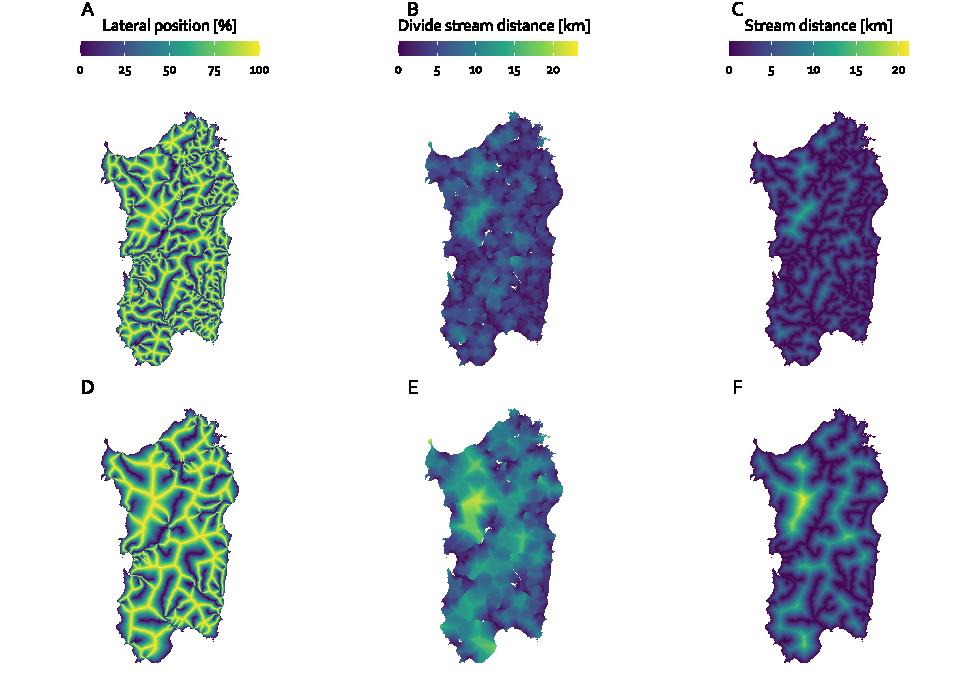
\includegraphics[width=1\linewidth]{data_descriptor/tex/figure-datasetmapoverviewplot-1} 

}

\caption{Resulting maps of the three EU-MOHP measures divide stream distance (A), lateral position (B),  and stream distance (C) in the columns exemplary for the three hydrologic orders 3 (1), 5 (2) and 7 (3) in the rows. Note the binned colour scale with breaks based on quantiles.}\label{fig:datasetmapoverviewplot}
\end{figure}

\normalsize

\small

\begin{figure}[H]

{\centering \includegraphics[width=0.7\linewidth]{data_descriptor/tex/workflow_figure} 

}

\caption{Workflow of the data processing in different software.}\label{fig:workflowfigure}
\end{figure}

\normalsize

\small

\begin{figure}[H]

{\centering \includegraphics[width=0.7\linewidth]{data_descriptor/tex/directory_tree} 

}

\caption{Directory tree of the project directory; only relevant subdirectories and files are listed here.}\label{fig:projectdirtree}
\end{figure}

\normalsize

\small

\begin{figure}[H]

{\centering \includegraphics[width=0.8\linewidth]{data_descriptor/tex/figure-dfddstatsbarplot-1} 

}

\caption{Distribution of the values in the attribute column dfdd.}\label{fig:dfddstatsbarplot}
\end{figure}

\normalsize

\small

\begin{figure}[H]

{\centering \includegraphics[width=1\linewidth]{data_descriptor/tex/mainstem_scheme} 

}

\caption{Schematic representation of the river network and its linestring geometries after import (A), after the identification of mainstems including the column levelpath\_id (B) and after merging the linestring geometries by this column and adding a feature\_id column (C).}\label{fig:mainstemscheme}
\end{figure}

\normalsize

\small

\begin{figure}[H]

{\centering \includegraphics[width=0.7\linewidth]{data_descriptor/tex/divergences_scheme} 

}

\caption{Schematic representation of the river network and its linestring geometries including divergences before (A) and after (B) the removal of minor paths under the condition that they intersect with the same linestring geometry at their start and end node. The linestring geometry with the feature\_id = 8 has been removed from the river network in B, because it intersects the linestring geometry with feature\_id = 1 at the start and end node. Whereas linestring geometry with feature\_id = 7 remains in the river network, because it intersects with two different linestring geometries at its start and end node.}\label{fig:divergencescheme}
\end{figure}

\normalsize

\small

\begin{figure}[H]

{\centering \includegraphics[width=0.8\linewidth]{data_descriptor/tex/figure-statsridgeplot-1} 

}

\caption{Ridgelines showing the distribution of the three measures DSD, LP and SD for all nine hydrologic orders.}\label{fig:statsridgeplot}
\end{figure}

\normalsize

\small

\begin{figure}[H]

{\centering \includegraphics[width=0.8\linewidth]{data_descriptor/tex/figure-rivercanalconfusionplot-1} 

}

\caption{Example of the river network data showing the confusion between the values BH140 (river), BH020 (canal) and BH030 (ditch) of the attribute column dfdd.}\label{fig:rivercanalconfusionplot}
\end{figure}

\normalsize

\small

\begin{figure}[H]

{\centering \includegraphics[width=0.7\linewidth]{data_descriptor/tex/dd_inaccuracies} 

}

\caption{Schematic example showing the source of inaccurate of DD in areas near headwaters caused by the applied method to calculate DD. The red distance as DD is incorrect, because it crosses the stream and therefore does not fulfill the defined condition. The correct DD would be the dark grey distance. The path to the correct side is equal to the correct DD (dark grey solid line) and therefore not drawn on the schematic map.}\label{fig:ddinaccuracies}
\end{figure}

\normalsize

\small

\begin{table}

\caption{\label{tab:runtime}Overview of the runtime and data size of all targets or processing steps in descending order.}
\centering
\begin{tabu} to \linewidth {>{\raggedright\arraybackslash}p{20em}>{\raggedleft}X>{\raggedleft}X>{\raggedleft}X>{\raggedleft}X>{\raggedleft}X}
\toprule
\multicolumn{1}{c}{ } & \multicolumn{4}{c}{Runtime} & \multicolumn{1}{c}{Data size} \\
\cmidrule(l{3pt}r{3pt}){2-5} \cmidrule(l{3pt}r{3pt}){6-6}
Target name & Seconds & Minutes & Hours & Days & Mb\\
\midrule
db\_objects\_to\_grass & 1199656.6 & 19994.3 & 333.2 & 13.9 & 0.0\\
rivernetworks\_merged\_per\_streamorder & 155852.7 & 2597.5 & 43.3 & 1.8 & 2002.6\\
eumohp\_files\_compression & 127353.4 & 2122.6 & 35.4 & 1.5 & 0.0\\
db\_inland\_waters\_strahler & 1741.6 & 29.0 & 0.5 & 0.0 & 0.0\\
river\_basins\_unioned & 1296.2 & 21.6 & 0.4 & 0.0 & 87.8\\
coastline\_unioned & 653.4 & 10.9 & 0.2 & 0.0 & 84.2\\
coastline\_buffer & 586.0 & 9.8 & 0.2 & 0.0 & 7.7\\
river\_basins\_subset\_union\_in\_db & 451.0 & 7.5 & 0.1 & 0.0 & 76.0\\
coastline\_filtered & 363.3 & 6.1 & 0.1 & 0.0 & 76.5\\
river\_networks & 235.3 & 3.9 & 0.1 & 0.0 & 1112.0\\
db\_river\_networks\_merged\_per\_streamorder & 835.3 & 13.9 & 0.2 & 0.0 & 0.0\\
db\_river\_networks\_clean & 129.9 & 2.2 & 0.0 & 0.0 & 0.0\\
inland\_waters & 101.4 & 1.7 & 0.0 & 0.0 & 183.0\\
db\_river\_networks\_strahler\_studyarea & 41.3 & 0.7 & 0.0 & 0.0 & 0.0\\
river\_networks\_clean & 38.0 & 0.6 & 0.0 & 0.0 & 1051.0\\
db\_inland\_waters & 25.6 & 0.4 & 0.0 & 0.0 & 0.0\\
river\_networks\_non\_dry\_selected\_streamtypes & 24.9 & 0.4 & 0.0 & 0.0 & 1053.7\\
rivernetworks\_feature\_id & 126.3 & 2.1 & 0.0 & 0.0 & 2070.1\\
river\_basins & 20.3 & 0.3 & 0.0 & 0.0 & 147.3\\
river\_basins\_subset & 8.7 & 0.1 & 0.0 & 0.0 & 84.0\\
streamorders & 5.7 & 0.1 & 0.0 & 0.0 & 0.0\\
coastline\_grouped & 5.4 & 0.1 & 0.0 & 0.0 & 92.8\\
quantile\_breaks & 5.1 & 0.1 & 0.0 & 0.0 & 0.0\\
config & 4.8 & 0.1 & 0.0 & 0.0 & 0.0\\
filepath\_coastline & 4.8 & 0.1 & 0.0 & 0.0 & 0.0\\
studyarea\_as\_coastline & 4.5 & 0.1 & 0.0 & 0.0 & 28.1\\
directory\_river\_networks & 4.5 & 0.1 & 0.0 & 0.0 & 0.0\\
coastline\_watershed & 4.2 & 0.1 & 0.0 & 0.0 & 29.8\\
db\_selected\_studyarea & 3.5 & 0.1 & 0.0 & 0.0 & 0.0\\
coastline\_buffer\_unioned & 3.1 & 0.1 & 0.0 & 0.0 & 7.5\\
selected\_studyarea & 2.0 & 0.0 & 0.0 & 0.0 & 29.8\\
major\_path\_ids & 1.9 & 0.0 & 0.0 & 0.0 & 4.4\\
bracket\_start\_ids & 1.7 & 0.0 & 0.0 & 0.0 & 0.0\\
river\_basins\_region\_name & 1.7 & 0.0 & 0.0 & 0.0 & 29.8\\
distinct\_streamorders\_in\_riverbasins & 1.1 & 0.0 & 0.0 & 0.0 & 0.0\\
river\_networks\_imputed\_streamorder\_canals\_as\_1 & 0.1 & 0.0 & 0.0 & 0.0 & 1053.7\\
rivernetworks\_merged\_per\_streamorder\_grouped & 0.0 & 0.0 & 0.0 & 0.0 & 2003.1\\
river\_networks\_files & 0.0 & 0.0 & 0.0 & 0.0 & 0.0\\
river\_basins\_grouped & 0.0 & 0.0 & 0.0 & 0.0 & 147.4\\
river\_basins\_files & 0.0 & 0.0 & 0.0 & 0.0 & 0.0\\
river\_basin\_names & 0.0 & 0.0 & 0.0 & 0.0 & 0.0\\
coastline\_regrouped & 0.0 & 0.0 & 0.0 & 0.0 & 84.2\\
river\_networks\_clip & 0.0 & 0.0 & 0.0 & 0.0 & 1112.0\\
\midrule
\textbf{Total} & \textbf{1489595.3} & \textbf{24826.6} & \textbf{413.7} & \textbf{17.2} & \textbf{12658.5}\\
\bottomrule
\end{tabu}
\end{table}

\normalsize

\small

\begin{table}

\caption{\label{tab:outputdata}Overview of the output file naming scheme and its placeholder values. Files for any combination of the placeholder values exists except for those study area polygons (<region name for spatial coverage>) that have no streams for certain hydrologic orders. The values are inserted for the respective placeholder in "mohp\_europe\_<region name for spatial coverage>\_<abbreviation of the EU-MOHP measure>\_<hydrologic order>\_<spatial resolution>.tif". For example, selecting the first value of each placeholder results in the file name "mohp\_europe\_europemainland\_dsd\_hydrologicorder1\_30m.tif". The spatial coverage of the values for "<region name for spatial coverage>" is shown in the mentioned interactive map in the Github repository.}
\centering
\begin{tabu} to \linewidth {>{\raggedright}X>{\raggedright\arraybackslash}p{12em}>{\raggedright}X}
\toprule
\multicolumn{1}{c}{Placeholder in output file name} & \multicolumn{1}{>{\centering\arraybackslash}p{12em}}{Value} & \multicolumn{1}{c}{Description}\\
\midrule
 & europemainland & Raster data covers the contiguous land area of continental Europe, ...\\
\cmidrule{2-3}
 & finland-norway-sweden & ...the Scandinavian countries Finland, Norway and Sweden\\
\cmidrule{2-3}
 & france & ...Corsica\\
\cmidrule{2-3}
 & greece & ...Creta\\
\cmidrule{2-3}
 & iceland & ...Iceland\\
\cmidrule{2-3}
 & italy1 & ...Sicily\\
\cmidrule{2-3}
 & italy2 & ...Sardinia\\
\cmidrule{2-3}
 & turkey & ...Turkey\\
\cmidrule{2-3}
 & unitedkingdom & ...United Kingdom\\
\cmidrule{2-3}
\multirow{-10}{*}{\raggedright\arraybackslash <region name for spatial coverage>} & unitedkingdom-ireland & Ireland and Northern Ireland\\
\cmidrule{1-3}
 & dsd & Divide stream distance\\
\cmidrule{2-3}
 & lp & Lateral Position\\
\cmidrule{2-3}
\multirow{-3}{*}{\raggedright\arraybackslash <abbreviation of the EU-MOHP measure>} & sd & Stream distance\\
\cmidrule{1-3}
 & streamorder1 & \\
\cmidrule{2-2}
 & streamorder2 & \\
\cmidrule{2-2}
 & streamorder3 & \\
\cmidrule{2-2}
 & streamorder4 & \\
\cmidrule{2-2}
 & streamorder5 & \\
\cmidrule{2-2}
 & streamorder6 & \\
\cmidrule{2-2}
 & streamorder7 & \\
\cmidrule{2-2}
 & streamorder8 & \\
\cmidrule{2-2}
\multirow{-9}{*}{\raggedright\arraybackslash <hydrologic order>} & streamorder9 & \multirow{-9}{*}{\raggedright\arraybackslash Hydrologic order}\\
\cmidrule{1-3}
<spatial resolution> & 30m & Spatial resolution\\
\bottomrule
\end{tabu}
\end{table}

\normalsize

\small

\begin{table}

\caption{\label{tab:statstabledata}Statistical summary of the calculated measures DSD, LP and SD across all hydrologic orders.}
\centering
\begin{tabu} to \linewidth {>{\centering\arraybackslash}p{7em}>{\raggedright}X>{\raggedright}X>{\raggedright}X>{\raggedright}X>{\raggedright}X>{\raggedright}X>{\raggedright}X>{\raggedright}X>{\raggedright}X>{\raggedright}X>{\raggedright}X>{\raggedright}X}
\toprule
\multicolumn{1}{c}{ } & \multicolumn{4}{c}{DSD} & \multicolumn{4}{c}{LP} & \multicolumn{4}{c}{SD} \\
\cmidrule(l{3pt}r{3pt}){2-5} \cmidrule(l{3pt}r{3pt}){6-9} \cmidrule(l{3pt}r{3pt}){10-13}
Hydrologic order & min & median & mean & max & min & median & mean & max & min & median & mean & max\\
\midrule
1 & 0.00 & 1.57 & 2.00 & 55.70 & 0 & 0.55 & 0.53 & 1 & 0 & 0.73 & 1.08 & 35.18\\
2 & 0.00 & 3.19 & 3.73 & 55.70 & 0 & 0.57 & 0.54 & 1 & 0 & 1.56 & 2.08 & 35.18\\
3 & 0.00 & 6.42 & 7.24 & 76.62 & 0 & 0.56 & 0.54 & 1 & 0 & 3.12 & 3.98 & 45.77\\
4 & 0.00 & 13.05 & 14.48 & 187.04 & 0 & 0.55 & 0.53 & 1 & 0 & 6.11 & 7.67 & 48.95\\
5 & 0.03 & 26.57 & 28.77 & 207.69 & 0 & 0.54 & 0.52 & 1 & 0 & 12.14 & 14.96 & 97.97\\
6 & 0.00 & 56.53 & 61.49 & 406.36 & 0 & 0.54 & 0.52 & 1 & 0 & 25.42 & 30.99 & 189.69\\
7 & 1.06 & 117.40 & 128.75 & 542.97 & 0 & 0.52 & 0.51 & 1 & 0 & 50.23 & 62.27 & 329.87\\
8 & 1.27 & 233.65 & 247.43 & 861.56 & 0 & 0.51 & 0.50 & 1 & 0 & 91.81 & 112.69 & 416.79\\
9 & 4.36 & 764.12 & 920.84 & 2526.04 & 0 & 0.17 & 0.28 & 1 & 0 & 129.17 & 159.96 & 561.65\\
\bottomrule
\end{tabu}
\end{table}

\normalsize

\renewcommand{\arraystretch}{2}

\small

\begin{table}

\caption{\label{tab:inputdata}Overview of the required input data to reproduce this dataset.}
\centering
\begin{tabu} to \linewidth {>{\raggedleft\arraybackslash}p{1em}>{\raggedright}X>{\raggedright}X>{\raggedright}X>{\raggedright}X>{\raggedright}X}
\toprule
No & Data layer & Data source & Layers in .gpkg files & Geometry type & Description\\
\midrule
1 & river network & EU-Hydro -- River Network Database & Canals\_l, Ditches\_l, River\_Net\_l & linestring & representing stream lines of rivers\\
2 & surface water bodies & EU-Hydro -- River Network Database & InlandWater & polygon & representing lakes, ponds and wide rivers\\
3 & river basins/ study area & EU-Hydro -- River Network Database & \_eudem2\_basins\_h1 & linestring & required to set the area for which the EU-MOHP measures are calculated for\\
4 & coastline & EU-Hydro -- Coastline & - & linestring & representing the coastline\\
\bottomrule
\end{tabu}
\end{table}

\normalsize

\renewcommand{\arraystretch}{1}
\FloatBarrier

\nocite{*}
\bibliography{eu-mohp.bib}

\end{document}
